In dependency of the Use Case of monitoring Hadoop cluster it is recommended to use Ambari or Chukwa. 
Both application were founded by Apache, which is also the creator of Hadoop. 
In archive each of them fulfils their range of use for monitoring processes properly. 
Ambari gives the user an overlook about all the technical details in Hadoop, and measures technical failures, while Chukwa is aimed on a supporting log handling on Hadoop. 
In conclusion can be sad that Ambari will support the whole use of Hadoop effectively in installation and running than Chukwa would be. 
Nevertheless there is not one right answer with of this applications is more useful for monitoring, because both differ very in their use-case field. 
A much more interesting Question would be, how Ambari and Chukwa could be used in a cooperation of their monitoring concepts.


\subsection{Summary}
This paper describes shortly the concept of monitoring on some current topics, especially in distributed scaled systems. As applications, that apply the concept of monitoring in distributed systems, Ambari and Chukwa were chosen. Those were explained by their architecture and use for the big data software Hadoop. In conclusion a use case for Chukwa was introduced more specific. 

\subsection{Use Case: Netflix}
\label{netflix}
One of the most known users of a \chuk derivate is \textbf{Netflix}, who is using \aws to provide their service. 
A fairly large number of \aws EC2 Instances is deployed, producing about $1.5$ million events per Second during peak hours. 
This results in about $80$ billion events per day. 
Most of the events are reflected as log messages, user activity records, system operational data, or any arbitrary data.~\cite{Bae2013}

Netflix is providing lots of its technology as Open-Source software, including their \chuk clone \textit{Suro}. 
Beside integrations with \noss, Suro offers several modifications to \chuk, which ``grew out of what [Netflix] learned from meeting the operational requirements of running in production over the past few years.''~\cite{Bae2013}

Suro goes beyond Chukwas scope of functionality in the following points:
\begin{enumerate}
  \item Suro supports ``arbitrary data formats,''~\cite{Bae2013} which allows more types of application to support advanced logging by Suro. A Plug-in System allows customised serialisation and deserialisation code to be run during processing.
  \item Lots of monitoring metrics are already included within Suro, 
  \item Integrations with other \noss Tools is included within Suro. This makes it especially easy to use Suro in a Cloud Setup, also using other \noss tools.~\cite{GithubNetflixSuro}
  \item \label{itm:SutoMultiDest} Dispatching Events to multiple destinations is available with custom configuration as of flexible architecture.~\cite{Bae2013, GithubNetflixSuro} A Message Router as described in Figure~\ref{fig:SuroMessageRouter} is used.
  \item ``Suro supports configurable store-and-forward on both client and collector.''~\cite{Bae2013} Its ``support of flexible retries'' leads to minimised data loss.~\cite{GithubNetflixSuro}
\end{enumerate}
Suro still preserves attributes from \chuk like horizontal scalability as well as ``large number of connections, and high throughput''~\cite{GithubNetflixSuro}

Item~\ref{itm:SutoMultiDest} allows Scenarios like the one described in Figure~\ref{fig:SuroArchitecture}. 
Here, every log message is still stored in a Data Sink File, which is stored on \aws S3 as Netflix is hosting in the \aws Environment, and then processed by Hadoop. But secondly, if the routing condition matches, the Event is also forwarded to Apache Kafka. Kafka will continue processing the log files and use other Services, like Druid and ElasticSearch, to create Bug Reports and send Notifications to Developers.
\begin{figure}[hbt]
  \centering
  % https://drive.google.com/open?id=1Nmn-mWvxAwhcB9Vo4nbq0gutnWp0bPcCfBU14KMDVQ8
  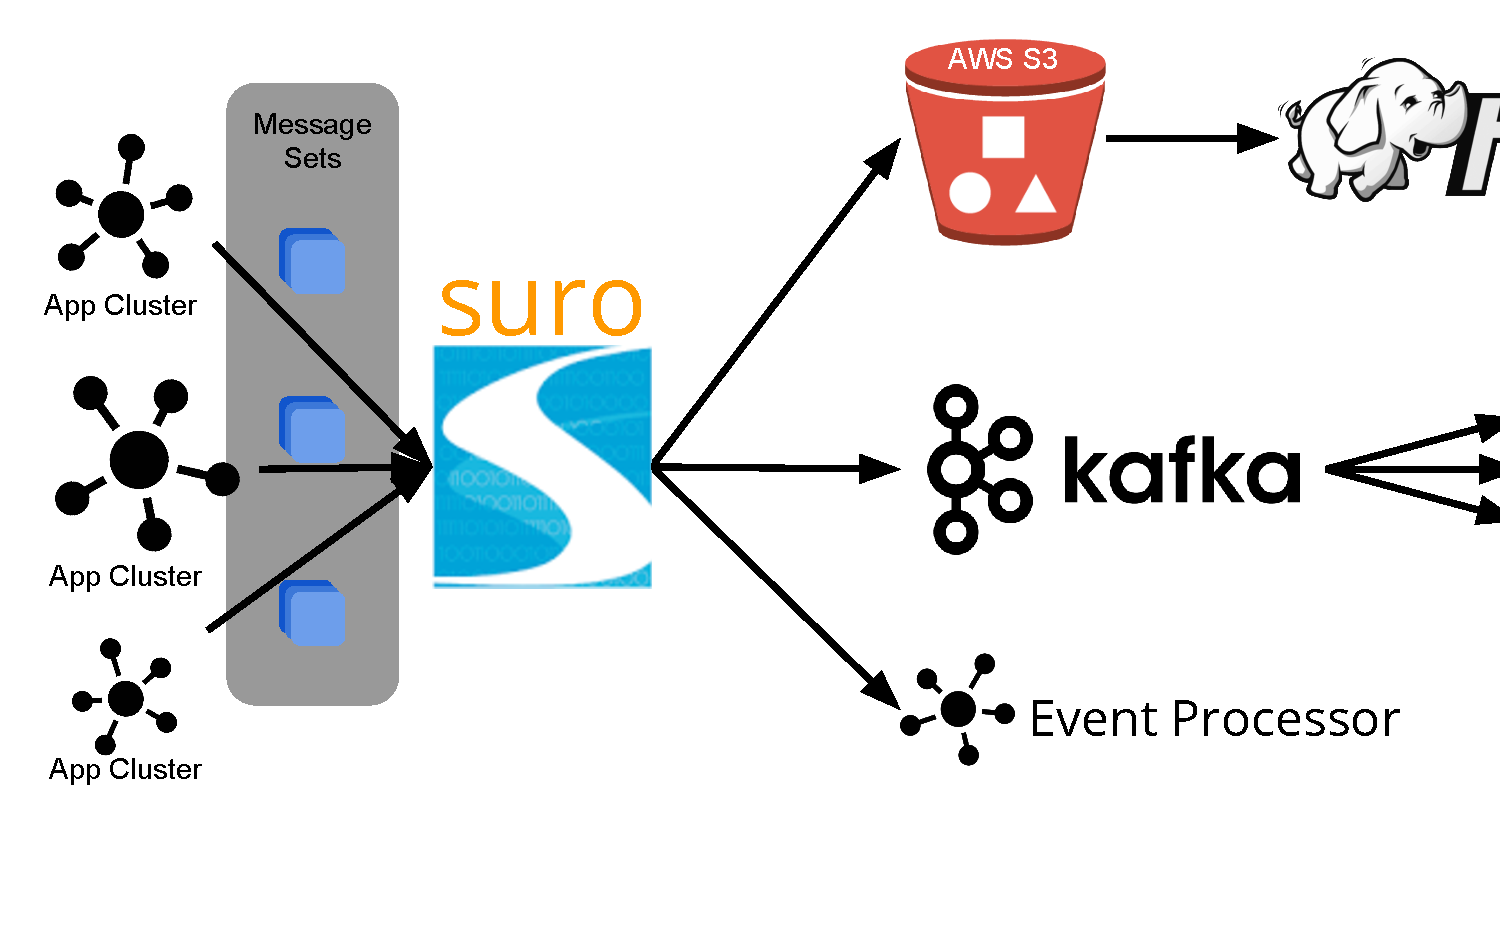
\includegraphics[width=\linewidth,clip=true,trim=5mm 2cm 0 5mm]{images/NetflixSuro}
  \caption{Netflix Suro Architecture~\cite{Bae2013, Harris2013}}
  \label{fig:SuroArchitecture}
\end{figure}


This routing is made possible by the Message Router that was Introduced with Suro (and which is not available with \chuk). On Figure~\ref{fig:SuroMessageRouter}, the Message Router is inserted between the Collector and the Storage. Also, different to \chuk (see Figure~\ref{fig:ChukwaArchitecture}) there are now multiple Storage modules that Events get routed to.
\begin{figure}[hbt]
  \centering
  % https://drive.google.com/open?id=1Nmn-mWvxAwhcB9Vo4nbq0gutnWp0bPcCfBU14KMDVQ8
  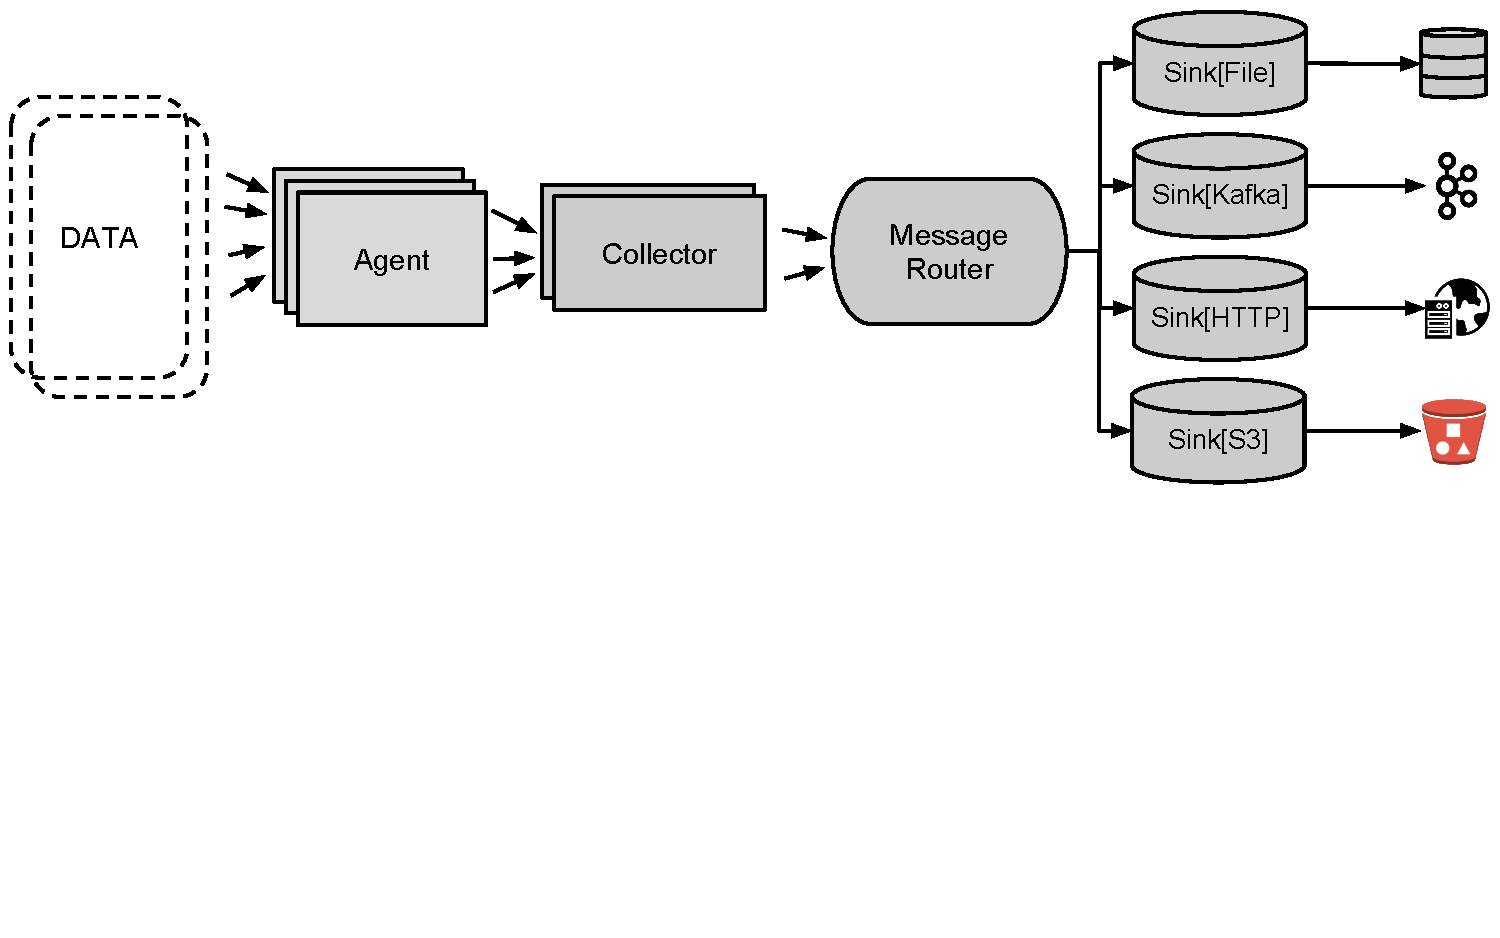
\includegraphics[width=\linewidth,clip=true,trim=0 75mm 0 0]{images/SuroMessageRouter}
  \caption{Netflix Suro Message Router~\cite{Bae2013}}
  \label{fig:SuroMessageRouter}
\end{figure}


\subsection{Future research}
Current research has not shown, in which extend the two systems \amblong and \chuk can be used in an inter-connected manner, complementing each others services. 
Managing large, internet-scale clusters, consisting of multiple thousand hosts running \hadooplong can be more automated and controlled with Systems like \amb and \chuk in place, not only controlling the current state, but also managing installed components and archiving system-state information.

Further, an improved way of storing Chukwas log data in a more structured way, allowing live querying, is still be to found. Boulon et al. did look into several options so far~\cite{Boulonb}, but this work has to be continued.

Last, but not least, the real-time approach shown in \ref{netflix} may be extended, as the ``recent trend has been in the area of real-time stream processing''~\cite{Bae2013} and will most likely continue in the future.